\documentclass{ctexart}

\usepackage{tikz}
\usepackage{tikzsymbols}
\usepackage{pgffor}
\usetikzlibrary {positioning}
\usetikzlibrary {math}
\tikzset{
boxA/.style={rectangle,minimum height=17pt,minimum width=20pt,draw=gray}
}
\tikzset{
boxB/.style={rectangle,minimum height=17pt,minimum width=30pt,draw=gray}
}
\tikzset{
boxC/.style={rectangle,minimum height=17pt,minimum width=120pt,draw=gray}
}
\begin{document}
\begin{tikzpicture}

\node[boxA] (A1) at (0,0) {1};
\foreach \i in {1,2,...,25}
{
\tikzmath{
int \j;
\j = \i+1;
}
\node[boxB,left=0 of A\i] (B\i) {};


\node[boxA,below=0 of A\i] (A\j) {\j};

\node[boxB,left=0 of A\j] (B\j) {};

}
%------------------------------------------------------------------------------------------------------------%
\node[boxC,right=0 of A1] (C1) {10MAA77CP101+};
%\draw (C1.east) -- ++(1,0);
\node[boxC,right=0 of A2] (C2) {10MAA77CP101-};
\draw[dashed] (B2) -- node[above left]{10MAA77CP101 1号汽轮机进口蒸汽压力1} ++(-2,0);
%------------------------------------------------------------------------------------------------------------%
\node[boxC,right=0 of A3] (C3) {10MAA77CP102+};
\node[boxC,right=0 of A4] (C4) {10MAA77CP102-};
\draw[dashed] (B4) -- node[above left]{10MAA77CP102 1号汽轮机进口蒸汽压力2} ++(-2,0);
%------------------------------------------------------------------------------------------------------------%
\node[boxC,right=0 of A5] (C5) {10MAA77CP103+};
\node[boxC,right=0 of A6] (C6) {10MAA77CP103-};
\draw[dashed] (B6) -- node[above left]{10MAA77CP103 1号汽轮机进口蒸汽压力3} ++(-2,0);

\end{tikzpicture}
\newpage
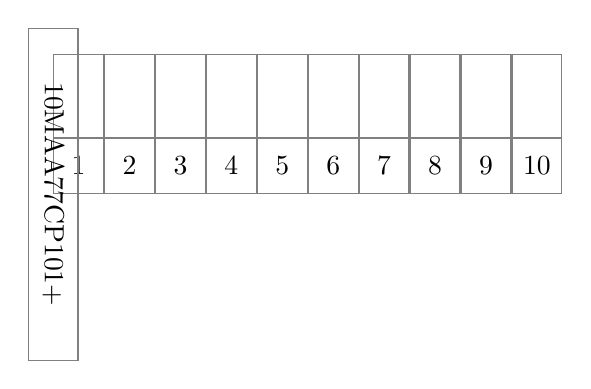
\begin{tikzpicture}[boxA/.style={rectangle,minimum height=20pt,minimum width=18pt,draw=gray},boxB/.style={rectangle,minimum height=30pt,minimum width=18pt,draw=gray},boxC/.style={rectangle,minimum height=18pt,minimum width=120pt,draw=gray}]

\node[boxA] (A1) at (0,0) {1};
\foreach \i in {1,2,...,9}
{
\tikzmath{
int \j;
\j = \i+1;
}
\node[boxB,above=0 of A\i] (B\i) {};


\node[boxA,right=0 of A\i] (A\j) {\j};

\node[boxB,above=0 of A\j] (B\j) {};

}
%------------------------------------------------------------------------------------------------------------%
%\node[boxC,below=0 of A1] (C1) {\parbox{1em}{10MAA77CP101+}};
\node[boxC,rotate=-90,below=0 of A1] (C1) {10MAA77CP101+};
%\draw (C1.east) -- ++(1,0);
%\node[boxC,rotate=90,below=0 of A2] (C2) {10MAA77CP101-};
%\draw[dashed] (B2) -- node[left]{\parbox{1em}{1号汽轮机进口蒸汽压力1}} ++(0,-2);

\end{tikzpicture}
\end{document}
